%%%%% Design %%%%%
\section{Design} 
This is the Design of the final report.
\subsection{Methodology}
\subsubsection{Forward Kinematics}
The manipulator consists of four sections, and the backbones of each section are perpendicular to each other. To derive the 
workspace of the manipulator for further analysis, the forward kinematics formula need to be conducted. According to the 
fishbone continuum robot\cite{fishboneCR}, the forward kinematics formula of two perpendicular sections are shown in 
Equations \ref{eq:x_coordinate}, \ref{eq:y_coordinate}, and \ref{eq:z_coordinate}.
\begin{align}
    \begin{aligned}
    x=&-\frac{S_{r}r}{\Delta S_{1}}+\frac{S_{r}r}{\Delta S_{1}}\cos\left(\frac{\Delta S_{l}}{r}\right)-d_{1}\sin\left(\frac{\Delta S_{l}}{r}\right) \\
    &-\frac{S_{r}r}{\Delta S_{3}}\sin\left(\frac{\Delta S_{1}}{r}\right)\sin\left(\frac{\Delta S_{3}}{r}\right) \\
    &-d_{2}\sin\left(\frac{\Delta S_{1}}{r}\right)\cos\left(\frac{\Delta S_{3}}{r}\right) 
    \end{aligned}
    \label{eq:x_coordinate}
\end{align}
\begin{align}
    \begin{aligned}
        y=-\frac{S_rr}{\Delta S_3}+\frac{S_rr}{\Delta S_3}\cos\left(\frac{\Delta S_3}{r}\right)-d_2\sin\left(\frac{\Delta S_3}{r}\right)
    \end{aligned}
    \label{eq:y_coordinate}
\end{align}
\begin{align}
    \begin{aligned}
        \text{Z} =&\frac{S_{r}r}{\Delta S_{1}}\sin\left(\frac{\Delta S_{\mathrm{l}}}{r}\right)+d_{1}\cos\left(\frac{\Delta S_{\mathrm{l}}}{r}\right) \\
        +&\frac{S_{r}r}{\Delta S_{3}}\sin\left(\frac{\Delta S_{3}}{r}\right)\cos\left(\frac{\Delta S_{1}}{r}\right) \\
        +&d_{2}\cos\left(\frac{\Delta S_{1}}{r}\right)\cos\left(\frac{\Delta S_{3}}{r}\right). 
    \end{aligned}
    \label{eq:z_coordinate}
\end{align}
However, calculating the centroid directly using the above formula becomes complex while there are four units in the manipulator. 
Additionally, the inverse kinematics part also requires the derivation of corresponding matrices for subsequent calculations 
using the composite coordinate transformation formula. Therefore, The relevant matrices for subsequent calculations need to 
be derived. \\
According to the design specifications, the manipulator comprises four units. The backbones of the units are vertically aligned. 
The base coordinate system can be established with the centroid of base disk upper surface serving as the origin. The x-axis of 
the coordinate system is aligned with the backbone of the unit nearest to the base disk. Consequently, the backbones of units 1 
and 3 are parallel to the x-axis, while those of units 2 and 4 are parallel to the y-axis. The positions of the five centroids 
in the base coordinate system when the manipulator is in the initial position are shown in Figure \ref{fig:kinematics model 0_0_0_0}. 
The centroids of the five disc upper surfaces are designated as $node_1$, $node_2$, $node_3$, $node_4$, and $node_5$. \\
\begin{figure}[H] %[H] "corresponds to start the figure Here" 
    \centering %alignment can be flushleft or flushright
    \captionsetup{labelsep=colon}
    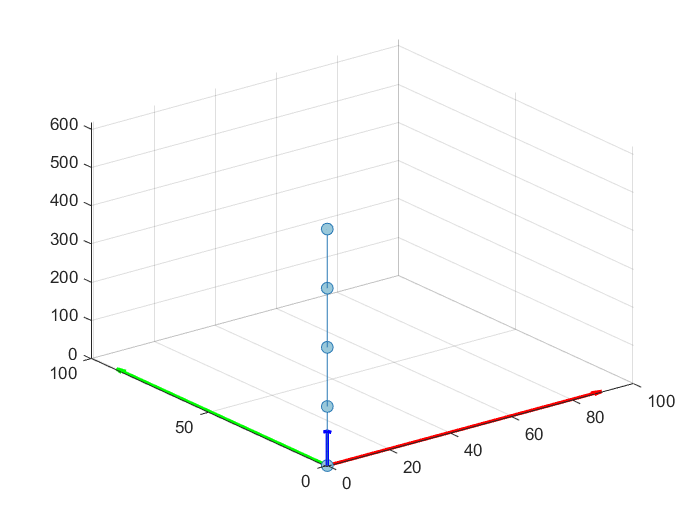
\includegraphics[width=1.0\textwidth]{Image/manipulator_0_0_0_0.png} 
    \caption[The kinematics model of manipulator in the initial position]
    {\centering \textit{\textbf{The kinematics model of manipulator in initial position.}}}
    \label{fig:kinematics model 0_0_0_0}
\end{figure}
\noindent The unit 1 is restricted to bending in the y-z plane of the coordinate system where $node_1$ serves as the origin, while the unit 2 
is restricted to bending in the x-z plane of the coordinate system where $node_2$ serves as the origin. Similarly, the unit 3 and 
unit 4 are subject to the same constraints. The bending angles for these units are defined as $\alpha_1$, $\alpha_2$, $\alpha_3$, 
and $\alpha_4$, respectively. The positions of the manipulator model in the base coordinate system after bending each unit by 
$90 \degree$ are illustrated in Figure \ref{fig:kinematics_model_resp}.
\begin{figure}[H] %[H] "corresponds to start the figure Here" 
    \centering %alignment can be flushleft or flushright
    \captionsetup{labelsep=colon}
    \begin{subfigure}{0.48\textwidth} % subfigure 1
        \centering
        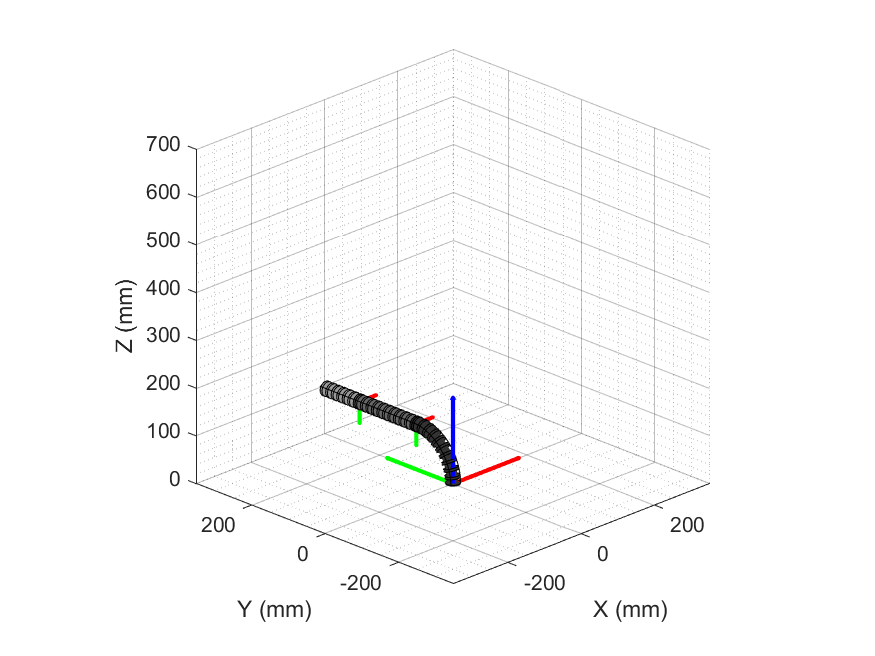
\includegraphics[width=\linewidth]{Image/manipulator_90_0_0_0.png}
        \caption{$\alpha_1=90 \degree,\alpha_2=0,\alpha_3=0,\alpha_4=0$}
    \end{subfigure}
    \hfill
    \begin{subfigure}{0.48\textwidth} % subfigure 2
        \centering
        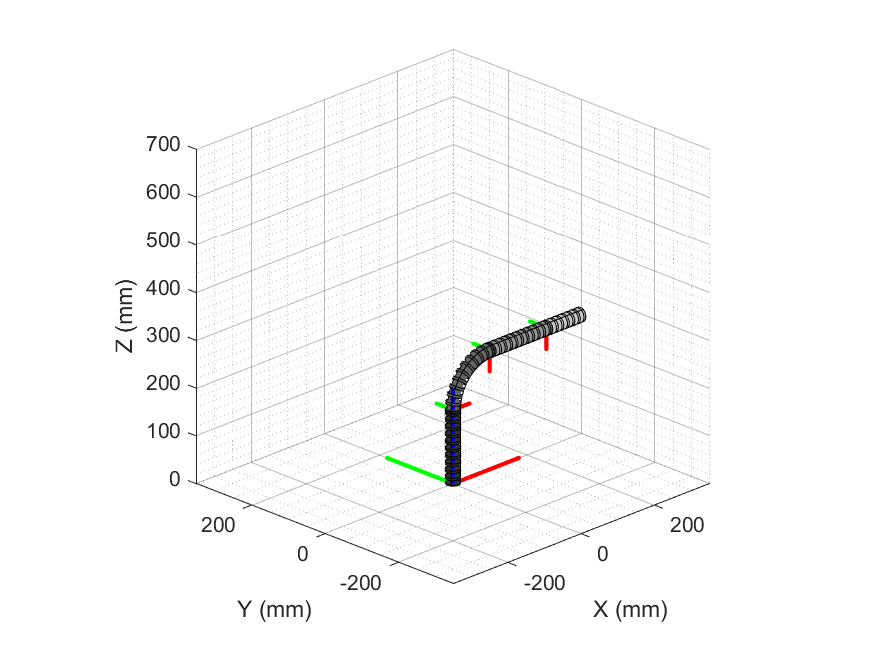
\includegraphics[width=\linewidth]{Image/manipulator_0_90_0_0.png}
        \caption{$\alpha_1=0,\alpha_2=90 \degree,\alpha_3=0,\alpha_4=0$}
    \end{subfigure}
    \begin{subfigure}{0.48\textwidth} % subfigure 3
        \centering
        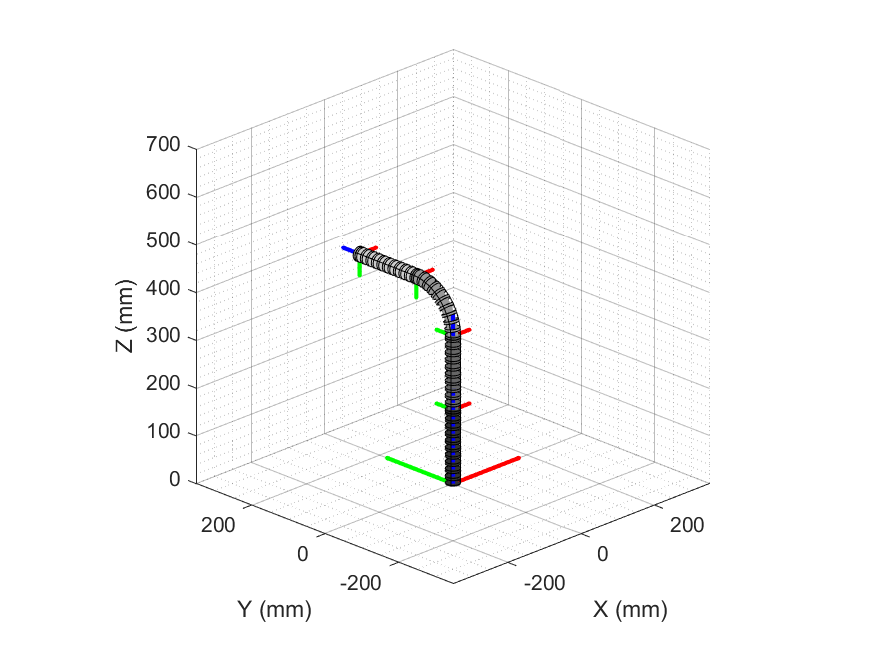
\includegraphics[width=\linewidth]{Image/manipulator_0_0_90_0.png}
        \caption{$\alpha_1=0,\alpha_2=0,\alpha_3=90 \degree,\alpha_4=0$}
    \end{subfigure}
    \hfill
    \begin{subfigure}{0.48\textwidth}
        \centering
        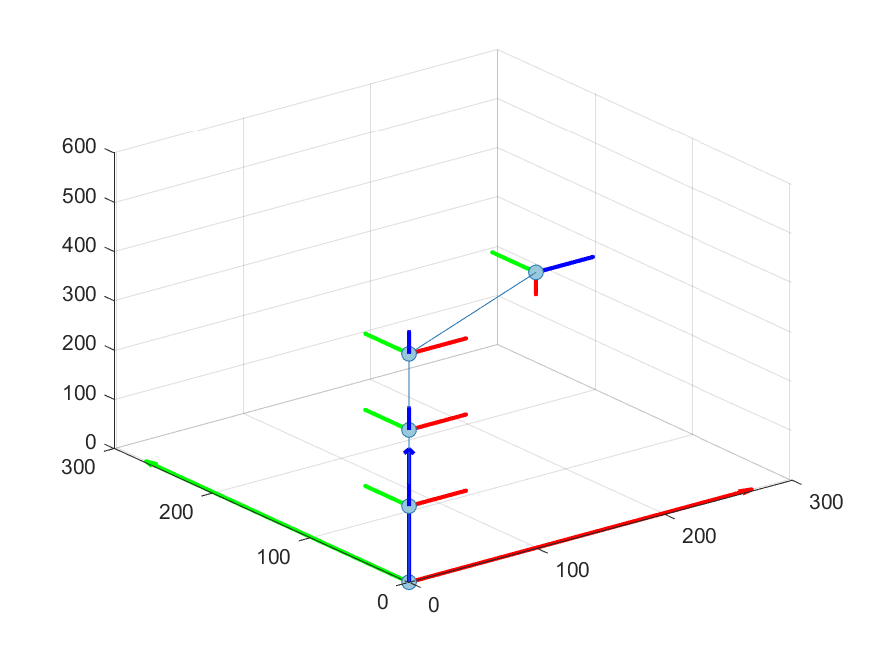
\includegraphics[width=\linewidth]{Image/manipulator_0_0_0_90.png}
        \caption{$\alpha_1=0,\alpha_2=0,\alpha_3=0,\alpha_4=90 \degree$}
    \end{subfigure}
    \caption[The kinematics model of manipulator with respective bending units]
    {\centering \textit{\textbf{The kinematics model of manipulator with respective bending units.}}}
    \label{fig:kinematics_model_resp}
\end{figure}
\noindent Owing to the distinct properties of the four units, different calculation methods are required for analysis. Therefore, 
the units are divided into odd and even groups for separate analysis. The unit $i$ have a base node $node_i$ and an end effector 
node $node_{i+1}$. To further calculate the position of $node_{i+1}$ in the base coordinate system, these matrices can be employed 
in the Equation \ref{eq:node i+1 calculation}.
\begin{align}
    &\textbf{P}_{i+1}^{base} = \textbf{B}_{i} \times \textbf{P}_{i+1}^{i} + \textbf{P}_{i}^{base}
    \label{eq:node i+1 calculation}
\end{align}
\begin{align*}
    &\ \textbf{P}_{i+1}^{base}\text{: The position of $node_{i+1}$ in the base coordinate system.}\\
    &\ \textbf{B}_{i}\text{: The rotational matrix tranforms the base coordinate system into coordinate}\\
    &\ \qquad\text{system \textit{i}, which is the coordinate system with origin $node_i$.}\\
    &\ \textbf{P}_{i+1}^{i}\text{: The position of $node_{i+1}$ in coordinate system \textit{i}.}\\
    &\ \textbf{P}_{i}^{base}\text{: The position of $node_{i}$ in the base coordinate system.}
\end{align*}
\begin{itemize}
    \item Unit 1
    \item Unit 2
    \item Unit 3
    \item Unit 4
\end{itemize}

The position of the end effector at the section whose backbone is parallel to the x-axis, which is $\textbf{P}_{end}$ can be 
derived based on the bending angle matrix $\textbf{B}$, mechanism parameters, the position of the end effector in the base 
coordinate system $\textbf{P}_{base}^{end}$ and the position of the base at the section $\textbf{P}_{base}$. The composite 
coordinate transformation is a combination of rotation and translation. The equations are shown in Equations \ref{eq:composite} 
and \ref{eq:composite_matrices}. $P_{horizontal}$ and $P_{vertical}$ are the horizontal and vertical position of end effector 
at the section in the base coordinate system, respectively. The sign of $P_{horizontal}$ in matrix $\textbf{P}_{base}^{end}$ 
consistent with the the sign of $\alpha$.
\begin{align}
    \textbf{P}_{end} = \textbf{B} \times \textbf{P}_{base} &+ \textbf{P}_{base}^{end} \label{eq:composite} \\
    \begin{bmatrix}
        x' \\
        y' \\
        z' \\
    \end{bmatrix}
    =
    \begin{bmatrix}
        1 & 0 & 0 \\
        0 & \cos(\alpha) & \sin(\alpha) \\
        0 & -\sin(\alpha) & \cos(\alpha) \\
    \end{bmatrix}
    &\times
    \begin{bmatrix}
        x \\
        y \\
        z \\
    \end{bmatrix}
    +
    \begin{bmatrix}
        0 \\
        \pm P_{\text{horizontal}} \\
        P_{\text{vertical}} \\
    \end{bmatrix}\label{eq:composite_matrices} \\
    P_{horizontal} = R\cdot(1-cos&(\alpha) + d\cdot cos(\alpha)) \nonumber \\ 
    P_{vertical} = R\cdot sin(\alpha) + &d\cdot sin(\alpha) \nonumber
\end{align}
The composite transfermation matrix of the first section whose backbone is parallel to x-axis is derived in Equations 
\ref{eq:CTMS1} and \ref{eq:composite_transf_matrix_section1}.
\begin{align}
    &\qquad\qquad
    \begin{aligned}
    \textbf{P}_{end,1}
    =
    \begin{bmatrix}
        \textbf{B}_1 & \textbf{P}_{base,1}^{end} \\
        \textbf{0} & 1 \\
    \end{bmatrix}
    \textbf{P}_{base,1}
    \end{aligned}\label{eq:CTMS1}\\
    &\begin{aligned}
    \begin{bmatrix}
        x' \\
        y' \\
        z' \\
        1  \\
    \end{bmatrix}
    =
    \begin{bmatrix}
        1 & 0 & 0 & 0 \\
        0 & cos(\alpha1) & sin(\alpha1) & \pm P_{horizontal,1} \\
        0 & -sin(\alpha1) & cos(\alpha1) & P_{vertical,1} \\
        0 & 0 & 0 & 1 \\
    \end{bmatrix}
    \begin{bmatrix}
        x \\
        y \\
        z \\
        1 \\
    \end{bmatrix}
    \end{aligned}
    \label{eq:composite_transf_matrix_section1}
\end{align}
The composite transfermation matrix of the second section whose backbone is parallel to y-axis is derived in Equations 
\ref{eq:CTMS2} and \ref{eq:composite_transf_matrix_section2}. ($\textbf{P}_{base,2}$ is equivalent to $\textbf{P}_{end,1}$)
\begin{align}
    &\qquad\qquad
    \begin{aligned}
    \textbf{P}_{end,2}
    =
    \begin{bmatrix}
        \textbf{B}_2 & \textbf{P}_{base,2}^{end} \\
        \textbf{0} & 1 \\
    \end{bmatrix}
    \textbf{P}_{base,2}
    \text{ ($\textbf{P}_{end,1}$)}
    \end{aligned}\label{eq:CTMS2}\\
    &\begin{aligned}
    \begin{bmatrix}
        x' \\
        y' \\
        z' \\
        1  \\
    \end{bmatrix}
    =
    \begin{bmatrix}
        cos(\alpha2) & 0 & sin(\alpha2) & \pm P_{horizontal,2} \\
        0 & 1 & 0 & 0 \\
        -sin(\alpha2) & 0 & cos(\alpha2) & P_{vertical,2} \\
        0 & 0 & 0 & 1 \\
    \end{bmatrix}
    \begin{bmatrix}
        x \\
        y \\
        z \\
        1 \\
    \end{bmatrix}
    \end{aligned}
    \label{eq:composite_transf_matrix_section2}
\end{align}
The manipulator consists of four sections. Therefore, the coordinates of the base and end effector of the manipulator can 
be expressed through the following forward kinematics matrices in Equation \ref{eq:FMplus4}.
\begin{align}
    \textbf{P}_{end,4}
    =
    \begin{bmatrix}
        \textbf{B}_4 & \textbf{P}_{base,4}^{end} \\
        \textbf{0} & 1 \\
    \end{bmatrix}
    \begin{bmatrix}
        \textbf{B}_3 & \textbf{P}_{base,3}^{end} \\
        \textbf{0} & 1 \\
    \end{bmatrix}
    \begin{bmatrix}
        \textbf{B}_2 & \textbf{P}_{base,2}^{end} \\
        \textbf{0} & 1 \\
    \end{bmatrix}
    \begin{bmatrix}
        \textbf{B}_1 & \textbf{P}_{base,1}^{end} \\
        \textbf{0} & 1 \\
    \end{bmatrix}
    \textbf{P}_{base,1}
    \label{eq:FMplus4}
\end{align}

\subsection{part ??}
unknown
\subsection{part ??}
unknown

% change to new page
\newpage